\documentclass[11pt, a4paper]{article}

\usepackage{amsmath}
\usepackage{amssymb}

% fonts
\usepackage{xeCJK}
\setCJKmainfont[BoldFont=SimHei]{SimSun}
\setCJKfamilyfont{hei}{SimHei}
\setCJKfamilyfont{kai}{KaiTi}
\setCJKfamilyfont{fang}{FangSong}
\newcommand{\hei}{\CJKfamily{hei}}
\newcommand{\kai}{\CJKfamily{kai}}
\newcommand{\fang}{\CJKfamily{fang}}

% style
\usepackage[top=2.54cm, bottom=2.54cm, left=3.18cm, right=3.18cm]{geometry}
\linespread{1.5}
\usepackage{indentfirst}
\parindent 2em
\punctstyle{quanjiao}
\renewcommand{\today}{\number\year 年 \number\month 月 \number\day 日}

% figures and tables
\usepackage{graphicx}
\usepackage[font={bf, footnotesize}, textfont=md]{caption}
\makeatletter
    \newcommand\fcaption{\def\@captype{figure}\caption}
    \newcommand\tcaption{\def\@captype{table}\caption}
\makeatother
\usepackage{booktabs}
\renewcommand\figurename{图}
\renewcommand\tablename{表}
\newcommand{\fref}[1]{\textbf{图\ref{#1}}}
\newcommand{\tref}[1]{\textbf{表\ref{#1}}}
\newcommand{\tabincell}[2]{\begin{tabular}{@{}#1@{}}#2\end{tabular}} % multiply lines in one grid

\usepackage{listings}
\lstset{basicstyle=\ttfamily}

\usepackage{xcolor}
\renewcommand{\r}{\color{red}}

\usepackage{url}

% tikz
\usepackage{tikz}
\usetikzlibrary{shapes.geometric, arrows}

\tikzstyle{actor} = [rectangle, rounded corners, minimum width=3cm, minimum height=1cm, text centered, draw=black, fill=red!30]
\tikzstyle{module} = [rectangle, minimum width=3cm, minimum height=1cm, text centered, draw=black, fill=orange!30]
\tikzstyle{arrow} = [thick,<->,>=stealth]

% start of document
\title{\textbf{\texttt{mydb}数据库设计报告}}
\author{\kai 朱俸民\quad 2012011894 
\and \kai 温和\quad 2013011407}
\date{\kai \today}

\begin{document}

\maketitle

\section{功能介绍}

\texttt{mydb}是一个简单的面向单用户、单线程的关系数据库管理系统,支持增、查、删、改四项基本数据库查询功能,通过SQL的一个子集实现数据库与用户的交互。除了支持基本的增、查、删、改功能外,\texttt{mydb}具有如下扩展功能:

\begin{enumerate}
    \item 索引:使用\texttt{std::set},支持对任意列建立索引加速查询;
    \item 域完整性约束:支持\texttt{CHECK}语句的创建,并在更新数据库时进行约束检查;
    \item 外键约束:支持\texttt{FOREIGN KEY}的创建,并在更新数据库时进行约束检查;
    \item 模糊查询:支持使用\texttt{LIKE}语句进行模糊匹配;
    \item 支持多表连接查询,包括三个表以上的连接;
    \item 聚集查询:支持将\texttt{SUM},\texttt{AVG},\texttt{MAX},\texttt{MIN}这四个函数应用于表中的某些列;
    \item 分组聚集查询:支持查询时的\texttt{GROUP BY}语句,可以处理聚集查询与分组聚集查询并存的查询;
    \item 完整的建表属性限制:建表时除了允许\texttt{NOT NULL},\texttt{PRIMARY KEY},\texttt{FOREIGN KEY}与\texttt{CHECK}限制外,还可以设置\texttt{UNIQUE},\texttt{AUTO\_INCREMENT}与\texttt{DEFAULT}限制;
    \item 在查询时,支持\texttt{BETWEEN}和\texttt{IN}操作符;
    \item 远程连接:允许远程开启\texttt{mydb}服务端后,本地用\texttt{mydb}客户端进行连接,通过SQL语句交互的方式进行数据库操作;
    \item 采用\texttt{MySQL}风格打印查询结果,易于用户查看。
\end{enumerate}

\section{系统架构}

\texttt{mydb}的顶层设计架构如\fref{arch}所示。

\begin{center}
    \begin{tikzpicture}[node distance=2cm]
        \node (user) [actor] {用户};
        \node (engine) [module, below of=user] {用户交互模块};
        \node (parse) [module, below of=engine] {SQL解析模块};
        \node (exe) [module, below of=parse] {SQL执行模块};
        \node (sys) [module, below of=exe] {系统管理模块};
        \node (record) [module, below of=sys] {记录管理模块};
        \node (table) [actor, left of=record, xshift=-2cm] {系统表};
        \node (config) [actor, right of=record, xshift=2cm] {配置文件};
        \node (fs) [actor, below of=record] {页式文件系统};
 
        \draw [arrow] (user) -- (engine);
        \draw [arrow] (engine) -- (parse);
        \draw [arrow] (parse) -- (exe);
        \draw [arrow] (exe) -- (sys);
        \draw [arrow] (sys) -- (record);
        \draw [arrow] (sys) -- (table);
        \draw [arrow] (sys) -- (config);
        \draw [arrow] (record) -- (fs);
    \end{tikzpicture}
    \fcaption{系统架构}\label{arch}
\end{center}

\section{模块设计}

\subsection{记录管理模块}

在数据存储上,某个数据库 (database) 的某一张表 (table) 对应于与数据库同名的目录下与表同名的一个文件。在访问该表时,调用提供的页式文件系统进行文件读写,其中,每页大小均为8KB。我们定义,该文件对应的各页中,第1页 (即编号为0的页) 存储与记录 (record) 相关的元数据,其数据格式如\tref{record:metadata}所示。

\begin{center}
    \tcaption{元数据记录格式}\label{record:metadata}
    \begin{tabular}{ll}
        \toprule
        偏移量 (字节) & 记录信息 \\
        \midrule
        0 & 每条记录长度 \\
        4 & 记录总个数 \\
        8 & 最后一条记录的ID (rid) \\
        12 & 最后一页的编号 (pid) \\
        1024 & 空闲页位图 \\
        \bottomrule
    \end{tabular}
\end{center}

其中,空闲页位图大小总计7K,用1表示空闲,0表示占用。之后的每一页,均用于存储各条记录的数据。这些页的前32字节为空闲位图,记录该页哪些位置处可以用来存放新的记录,共计256位,分别对应该页的每32个字节 (称为一个\textbf{字}) 是否可用。因此,所有的记录必须按一个字对齐。对于具有$n$列的一条记录,其数据格式如\tref{record:record}所示。

\begin{center}
    \tcaption{记录数据格式}\label{record:record}
    \begin{tabular}{ll}
        \toprule
        偏移量 (字节) & 记录信息 \\
        \midrule
        0 & 记录ID (rid)  \\
        4 & 各字段是否为空的位图 \\
        $4+n$ & 记录的数据 \\
        \bottomrule
    \end{tabular}
\end{center}

对于记录的数据,我们按照列的顺序依次存储,我们支持如\tref{record:types}所示的数据类型。

\begin{center}
    \tcaption{支持的数据类型}\label{record:types}
    \begin{tabular}{lll}
        \toprule
        类型 & 映射的C++类型 & 长度 (字节) \\
        \midrule
        BOOL & \texttt{bool} & 1 \\
        SHORT & \texttt{int8\_t} & 2 \\
        INT & \texttt{int16\_t} & 4 \\
        LONG & \texttt{int32\_t} & 8 \\
        FLOAT & \texttt{float} & 4 \\
        DOUBLE & \texttt{double} & 8 \\
        CHAR & \texttt{char} & 1 \\
        STRING & \texttt{char*} & 最大65535 \\
        \bottomrule
    \end{tabular}
\end{center}

每条记录的数据部分最长支持65535字节。

\subsection{系统管理模块}

!TODO

\subsection{SQL解析模块}

我们利用了\texttt{flex}和\texttt{bison}工具构建SQL语句解析前端,将SQL语句转换为自定义的语法树结构。对于语法正确的语句,我们采用Visitor设计模式,对其进行遍历,检查可能出现的类型不一致、数量不一致等错误。然后将其送往SQL执行模块执行,并获取执行后返回的结果。若执行成功,利用\texttt{MySQL}风格 (如\fref{myprint}) 打印出查询结果;否则,打印出错误信息。

\begin{center}
    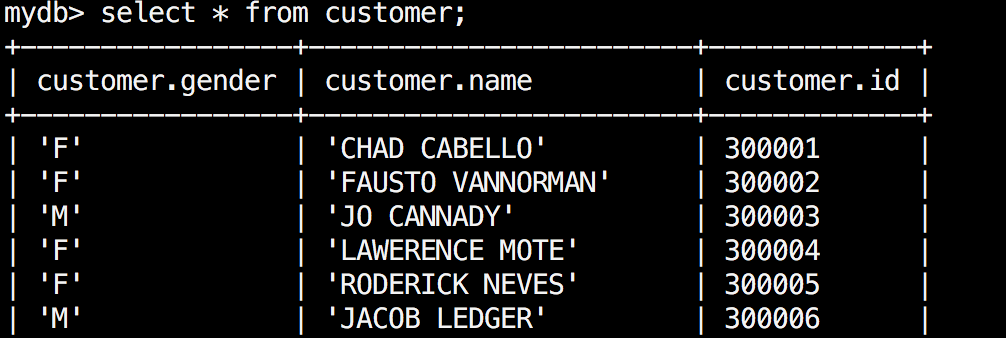
\includegraphics[width=11cm]{fig/mysql}
    \fcaption{\texttt{MySQL}风格打印}\label{myprint}
\end{center}

接下来我们列出\texttt{mydb}支持的SQL。

\subsubsection{\texttt{mydb}关键字}

\subsubsection{\texttt{mydb}文法}

\subsubsection{\texttt{mydb}运算符优先级}

\subsection{SQL执行模块}

!TODO

\subsection{用户交互模块}

在顶层,我们设计了一个交互式终端,方便用户键入SQL语句并执行数据库操作。输入\texttt{exit}或\texttt{quit}可以退出终端。我们还支持多行输入SQL语句  (如\fref{inter:multi}),以\texttt{;}作为语句的结束。

\begin{center}
    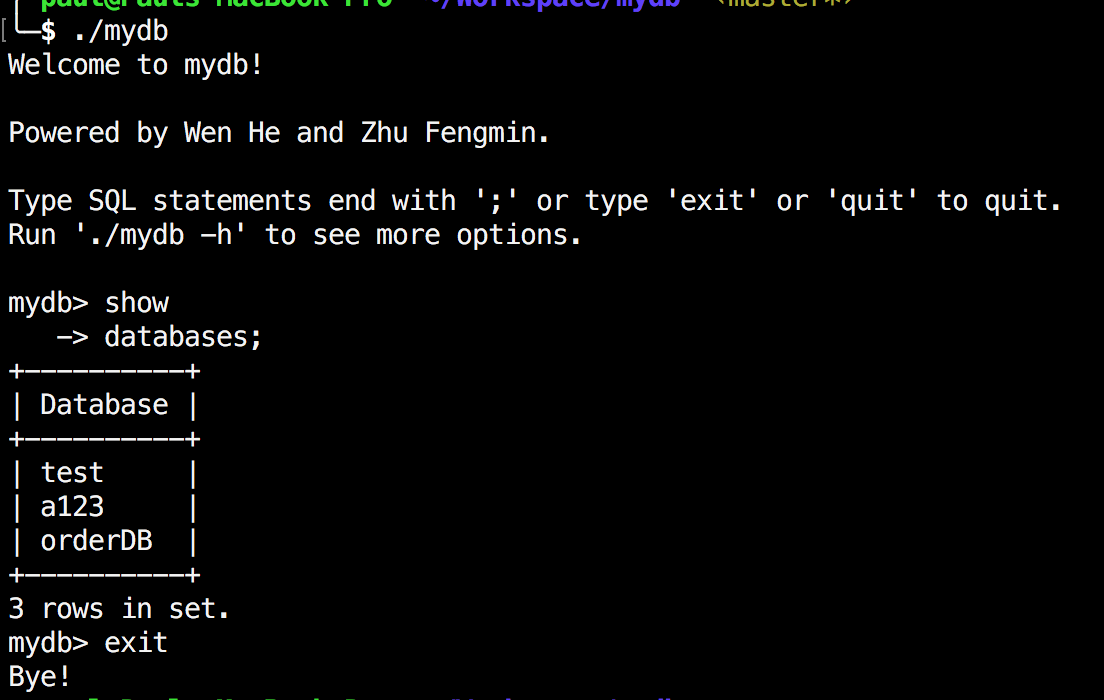
\includegraphics[width=11cm]{fig/multi-row}
    \fcaption{交互式终端允许多行输入}\label{inter:multi}
\end{center}

\section{测试结果}

\subsection{基本查询功能}

!TODO

\subsection{扩展查询功能}

!TODO

\subsection{远程连接功能}

首先,我们启动一个服务端。

\begin{center}
    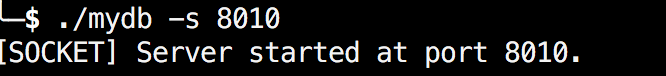
\includegraphics[width=8cm]{fig/server}
    \fcaption{启动服务端}
\end{center}

接下来,我们通过客户端连接服务端。

\begin{center}
    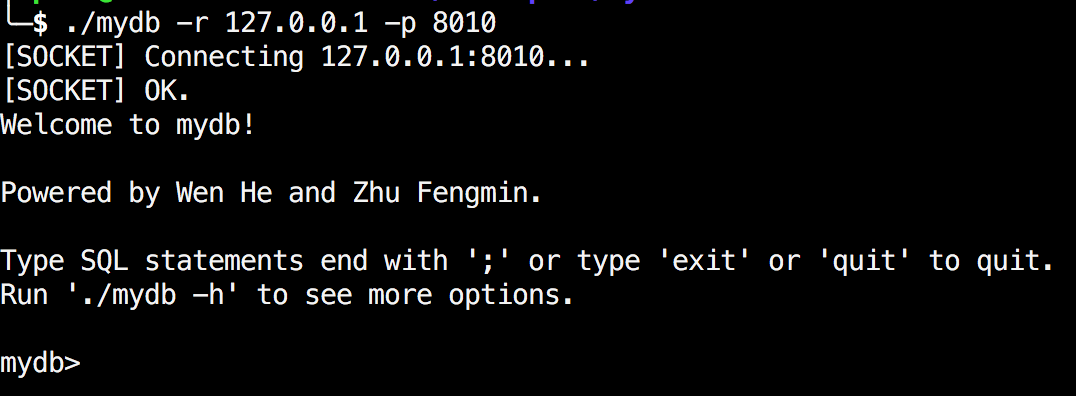
\includegraphics[width=11cm]{fig/conn}
    \fcaption{客户端连接服务端}
\end{center}

最后,我们输入一系列SQL语句,测试服务端返回的信息都是正确的。

\begin{center}
    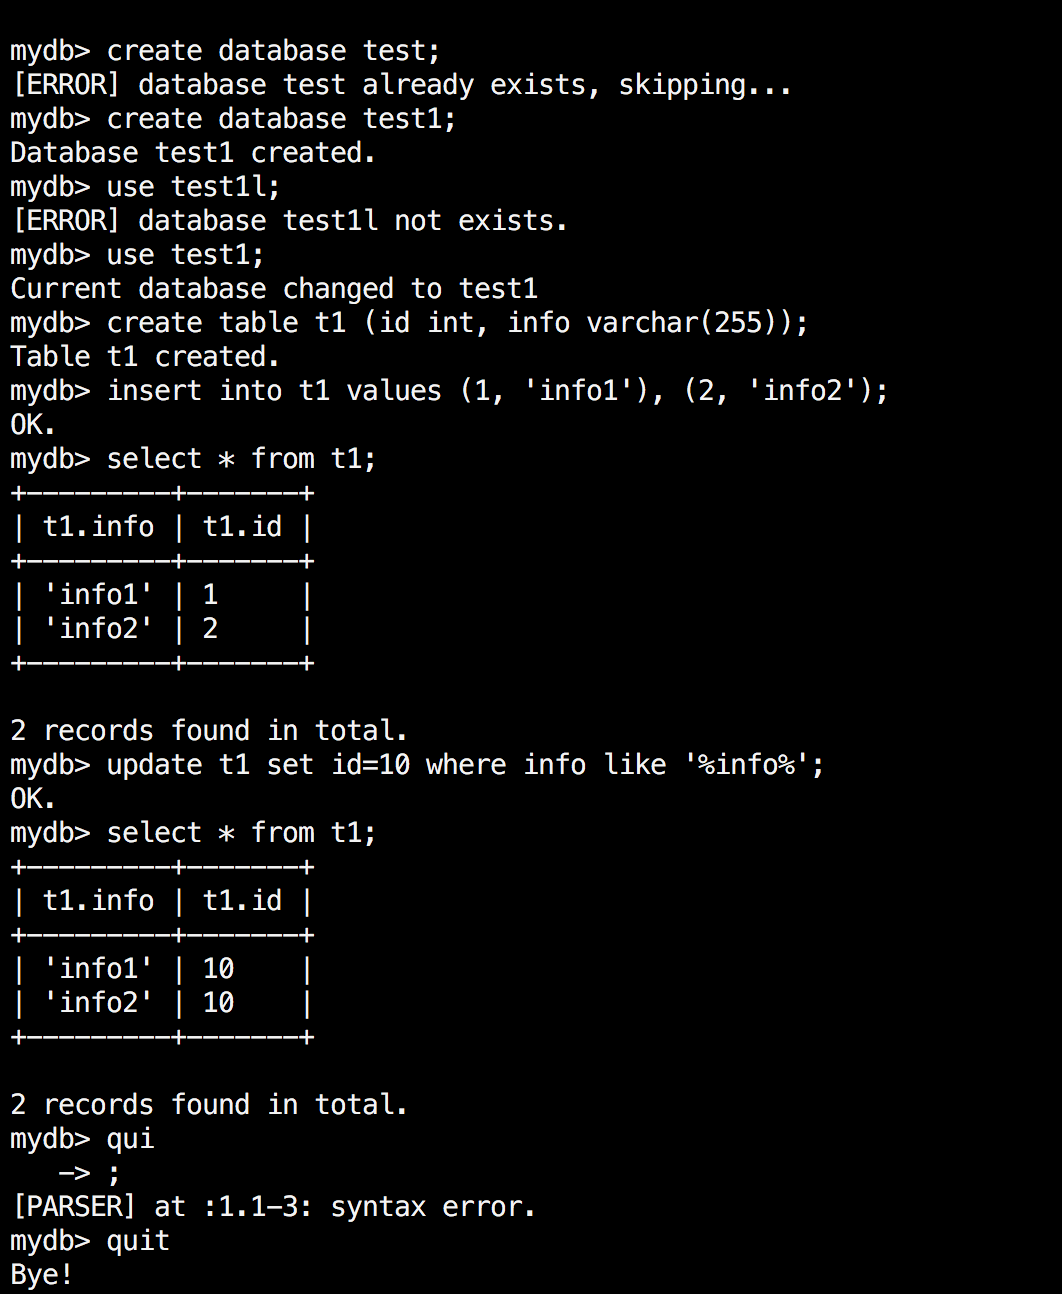
\includegraphics[width=11cm]{fig/conn-test}
    \fcaption{远程操作数据库}
\end{center}

退出客户端后,服务端仍然等待新的客户端连接。

\begin{center}
    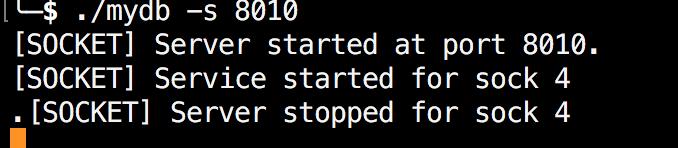
\includegraphics[width=8cm]{fig/disconn}
    \fcaption{断开连接}
\end{center}

\section{小组分工}

请见\tref{jobs}。

\begin{center}
    \tcaption{小组分工}\label{jobs}
    \begin{tabular}{ll}
        \toprule
        功能 & 负责人 \\
        \midrule
        记录管理 & 朱俸民 \\
        系统管理 & 温和 \\
        SQL解析与语义检查 & 朱俸民 \\
        查询执行 & 温和 \\
        交互终端与远程连接 & 朱俸民 \\
        索引 & 温和 \\
        \bottomrule
    \end{tabular}
\end{center}

\section{使用方法}

详见\texttt{README.md},或前往Github:\url{https://github.com/paulzfm/mydb#mydb}。



\begin{thebibliography}{9}

\bibitem{bib1} Bison 2.3. \url{https://engineering.purdue.edu/~milind/ece573/2015fall/project/bison.html#Calc_002b_002b-_002d_002d_002d-C_002b_002b-Calculator}.

\bibitem{bib2} SQL Tutorial. \url{http://www.w3schools.com/sql/default.asp}.

\bibitem{bib3} 冯建华, 周立柱. 数据库系统设计与原理. 

\bibitem{bib4} cppreference. \url{http://en.cppreference.com/}.

\bibitem{bib5} RapidJSON. \url{http://rapidjson.org/index.html}.

\end{thebibliography}

\end{document}
